\chapter{Simulation}
\label{chap6}
Circuit simulation \index{Circuit simulation} uses mathematical models to replicate the behaviour of an actual device or circuit. Simulation software allows for modeling of circuit operation. Simulating a circuit's behaviour before actually building it can greatly improve design efficiency by making faulty designs known as such, and providing insight into the behavior of electronic circuit designs. Oscad uses {\tt Ngspice}\index{Ngspice} for mixed-level/mixed-signal circuit simulation. 

The various steps involved in simulating a circuit schematic in Oscad is given below:
\begin{enumerate}
\item Analysis insertion \index{Analysis insertion} - This adds the type of simulation to be done to the netlist. This is done by the {\tt Analysis inserter} tool in the Oscad tool bar.
\item Netlist conversion \index{KiCad to Ngspice conversion} - The netlist created in the Schematic editor will be converted to Ngspice format and analysis options will be appended to it. This is done by the {\tt Netlist Converter} tool in the Oscad tool bar.
\item Ngspice simulation \index{Ngspice simulation} - Ngspice simulation of the netlist is performed. This is done by the {\tt Ngspice} tool in the Oscad tool bar.
\end{enumerate}

In the following sections, we shall describe each of the above steps.
\section{Analysis Inserter} \index{Analysis Inserter}
\label{ana}
In order to simulate a circuit, the user must define the type of analysis to be done on the circuit. The types of analysis \index{Types of Analysis} include Operating point analysis, DC analysis, AC analysis, transient analysis etc. The user should also specify the options corresponding to each analysis. This is facilitated by the {\tt Analysis inserter} tool in Oscad.

Analysis inserter generates the commands for Ngspice. When you click on analysis inserter from the Oscad tool bar, you will get the Analysis inserter GUI as shown in Figure \ref{1}. It consists of type of analysis on the top, and user needs to type the details which are needed to perform simulation in the corresponding fields.
\subsection{Types of Analysis} \index{Types of Analysis}
Oscad supports three types of analyses:
\begin{enumerate}
\item DC Analysis (Operating Point and DC Sweep) \index{DC Analysis}
\item AC Small-signal Analysis \index{AC Small-signal Analysis} 
\item Transient Analysis \index{Transient Analysis}
\end{enumerate}
Other analyses in the Analysis inserter are currently under progress.
The different types of analyses supported in Oscad are explained below \cite{ngspice}.
\subsubsection{DC Analysis} \index{DC Analysis}
The dc analysis determines the dc operating point of the circuit with inductors shorted and capacitors opened. The dc analysis options are specified on the {\tt .dc} \index{.dc}, and {\tt .op}\index{.op} control lines. 

There is assumed to be no time dependence on any of the sources within the system description. The simulator algorithm subdivides the circuit into those portions which require the analog simulator algorithm and those which require the event-driven algorithm. Each subsystem block is then iterated to solution, with the interfaces between analog nodes and event-driven nodes iterated for consistency across the entire system. 

Once stable values are obtained for all nodes in the system, the analysis halts and the results may be displayed or printed out as you request them.
 
A dc analysis is automatically performed prior to a transient analysis to determine the transient initial conditions, and prior to an ac small-signal analysis to determine the linearized, small-signal models for nonlinear devices. 
 The dc analysis can also be used to generate dc transfer curves: a specified independent voltage or current source is stepped over a user-specified range and the dc output variables are stored for each sequential source value. 
\subsubsection{AC Small-signal Analysis}\index{AC Small-signal Analysis}
AC analysis is limited to analog nodes and represents the small signal, sinusoidal solution of the analog system described at a particular frequency or set of frequencies. This analysis is similar to the DC analysis in that it represents the steady-state behavior of the described system with a single input node at a given set of stimulus frequencies. 

The program first computes the dc operating point of the circuit and determines linearized, small-signal models for all of the nonlinear devices in the circuit. The resultant linear circuit is then analyzed over a user-specified range of frequencies. The desired output of an ac small-signal analysis is usually a transfer function (voltage gain, transimpedance, etc). If the circuit has only one ac input, it is convenient to set that input to unity and zero phase, so that output variables have the same value as the transfer function of the output variable with respect to the input.
\subsubsection{Transient Analysis}\index{Transient Analysis}
Transient analysis is an extension of DC analysis to the time domain. A transient analysis begins by obtaining a DC solution to provide a point of departure for simulating time-varying behavior. Once the DC solution is obtained, the time-dependent aspects of the system are reintroduced, and the simulator algorithms incrementally solve for the time varying behavior of the entire system. Inconsistencies in node values are resolved by the simulation algorithms such that the time-dependent waveforms created by the analysis are consistent across the entire simulated time interval.

 Resulting time-varying descriptions of node behavior for the specified time interval are accessible to you. All sources which are not time dependent (for example, power supplies) are set to their dc value. The transient time interval is specified on a {\tt .tran} control line. 


\begin{figure}[t]
\centering
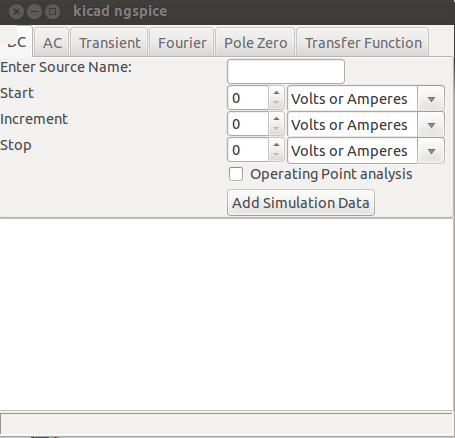
\includegraphics[width=0.5\textwidth]{figures/1}
\caption{Analysis inserter GUI}
\label{1}
\end{figure}
\subsection{DC Analysis Inserter}
By default DC analysis option will appear when you click on analysis inserter. Here we need to give the details of input source name, start value of input, increment and  stop value. Then click on ``Add Simulation Data". 

The Figure \ref{2} gives an example of DC analysis inserter.
\begin{figure}[t]
\centering
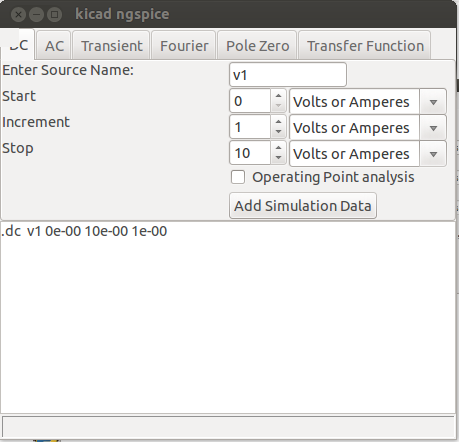
\includegraphics[width=0.5\textwidth]{figures/2}
\caption{DC Analysis option added}
\label{2}
\end{figure}
In this example 'v1' is the input voltage source which starts at '0 Volt', increments by '1 Volt' and stops at '10 Volt'. On clicking ``Add simulation data", the analysis statement is generated and is of the form:

\textit{.dc\index{.dc} sourcename vstart vstop vincr}

The {\tt .dc} line defines the dc transfer curve source and sweep limits (with capacitors open and inductors shorted). {\tt srcnam} is the name of an independent voltage or current source. {\tt vstart, vstop}, and {\tt vincr} are the starting, final, and incrementing values respectively, of the source.

When we check the option {\tt Operating point analysis}\index{Operating point analysis} on the DC analysis window, {\tt .op} gets appended to the analysis statement. This is shown in Figure \ref{3}.
\begin{figure}[t]
\centering
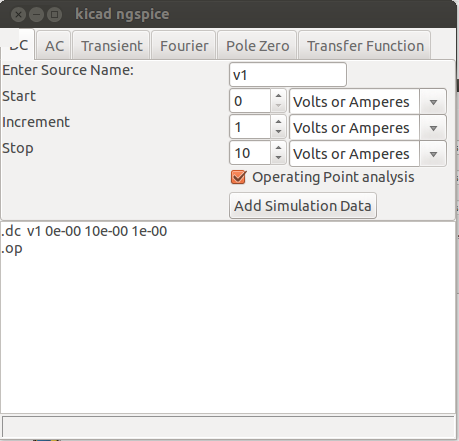
\includegraphics[width=0.5\textwidth]{figures/3}
\caption{OP Analysis}
\label{3}
\end{figure}
The inclusion of the line {\tt .op} in the analysis file directs Ngspice to determine the dc operating point of the circuit with inductors shorted and capacitors opened. 
\subsection{AC Analysis Inserter}\index{AC Analysis Inserter}
When you click on the option ``AC" in the analysis inserter GUI, the window given in Figure \ref{4} will appear.
\begin{figure}[t]
\centering
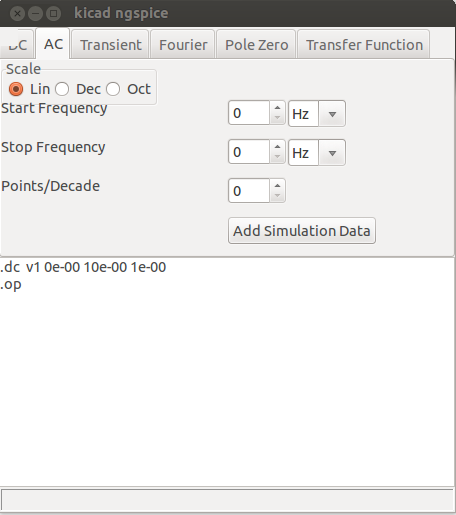
\includegraphics[width=0.5\textwidth]{figures/4}
\caption{AC Analysis GUI}
\label{4}
\end{figure}
Here you need to enter the details of {\tt scale}, {\tt start frequency}, {\tt stop frequency} and {\tt Number of points}.

After entering these values, click on ``Add Simulation Data". The analysis statement will be generated. This will be in one of the three forms listed below, depending on the type of {\tt scale} that you choose. The types of {\tt scale} available are dec, oct, and lin. \\
{\tt .ac dec nd fstart fstop }\\ \index{.ac}
{\tt .ac oct no fstart fstop }\\
{\tt .ac lin np fstart fstop }

{\tt dec} stands for decade variation, and {\tt nd} is the number of points per decade. {\tt oct} stands for octave variation, and {\tt no} is the number of points per octave. {\tt lin} stands for linear variation, and np is the number of points. {\tt fstart} is the starting frequency, and {\tt fstop} is the final frequency. 

If the {\tt .ac} analysis is included in the analysis file, Ngspice performs an AC analysis of the circuit over the specified frequency range. Note that in order for this analysis to be meaningful, at least one independent source must have been specified with an ac value.

An example of ``lin" scale is given in Figure \ref{5}.
\begin{figure}[t]
\centering
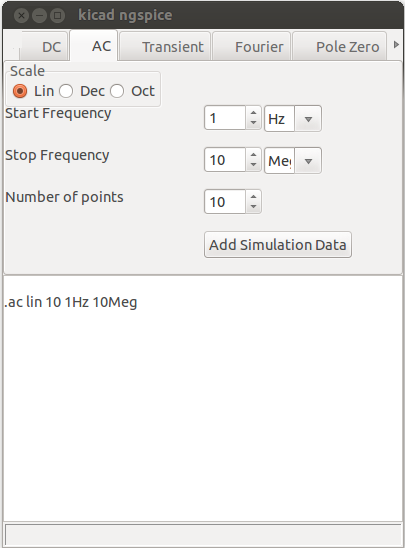
\includegraphics[width=0.5\textwidth]{figures/5}
\caption{AC Analysis options added}
\label{5}
\end{figure}
Here the start frequency is ``1 Hz", stop frequency is ``10 Meg" and  number of points is ``10".

\subsection{Transient Analysis Inserter}\index{Transient Analysis Inserter}
When you click on the option ``Transient" in the analysis inserter GUI, the window
given in Figure \ref{6} will appear. Here you need to enter the details of {\tt start time}, {\tt step time}, and {\tt stop time}.
After entering these values, click on “Add Simulation Data”. The analysis
statement will be generated. It will be of the form:

{\tt .tran tstep tstop tstart}\index{.tran}

{\tt tstep} is the printing or plotting increment for line-printer output. For use with the postprocessor, {\tt tstep} is the suggested computing increment. {\tt tstop} is the final time, and {\tt tstart} is the initial time. If tstart is omitted, it is assumed to be zero.

 The transient analysis always begins at time zero. In the interval $\textless$ zero, tstart $\textgreater$, the circuit is analyzed (to reach a steady state), but no outputs are stored. In the interval $\textless$ tstart, tstop $\textgreater$, the circuit is analyzed and outputs are stored. 

\begin{figure}[t]
\centering
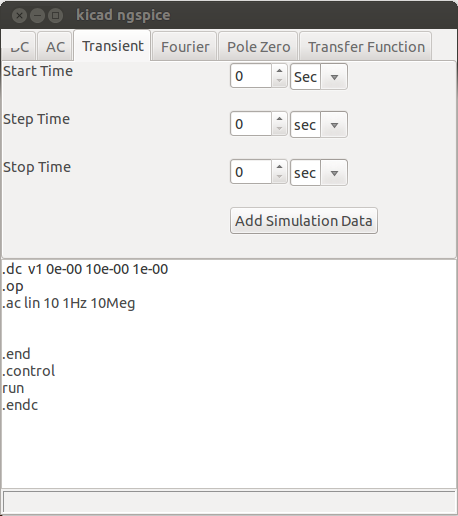
\includegraphics[width=0.5\textwidth]{figures/6}
\caption{Transient Analysis - GUI}
\label{6}
\end{figure}
 \begin{figure}[t]
\centering
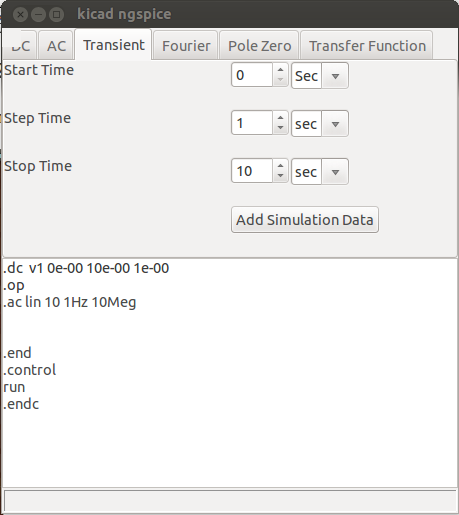
\includegraphics[width=0.5\textwidth]{figures/7}
\caption{Transient Analysis options added}
\label{7}
\end{figure}
An example of transient analysis inserter is given in Figure \ref{7}.
Here start time is ``0 sec", step time is ``1 sec" and stop time is ``10 sec".

\subsection{Saving the analysis file}
After entering the details of analysis we need to save the {\tt analysis} file, which contains the options we added. Save the analysis file as explained below:

Click on ``File" from the top menu bar. Click on ``Save". This is shown in Figure \ref{8-file}. Click on Save in the {\tt Choose a File} dialog box as shown in Figure \ref{8-save}. The options added in the analysis inserter GUI will be saved in a file named {\tt analysis}. 
\begin{figure}[t]
\centering
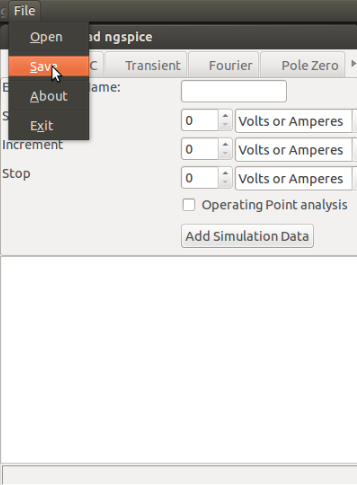
\includegraphics[width=0.5\textwidth]{figures/8-file}
\caption{Choosing the Save option from File menu}
\label{8-file}
\end{figure}

\begin{figure}[t]
\centering
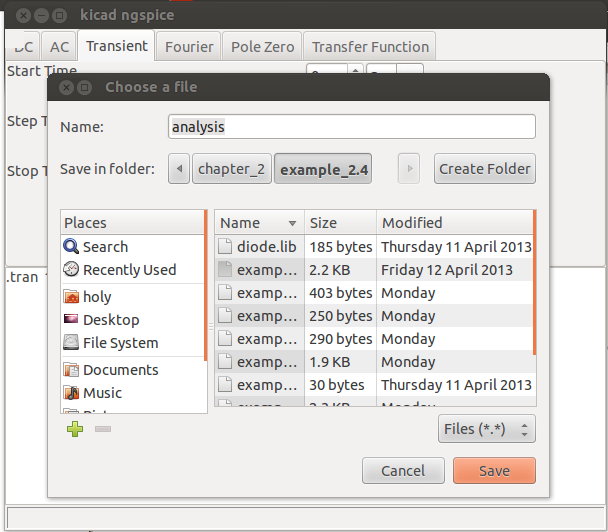
\includegraphics[width=0.7\textwidth]{figures/8-save}
\caption{Saving the analysis information to netlist}
\label{8-save}
\end{figure}
\section{Modifying KiCad netlist for Ngspice simulation} \index{Netlist converter}
The schematic editor provides a netlist file, which describes the electrical connections between circuit components. This is a SPICE netlist \index{SPICE netlist} which can not be directly used for Ngspice simulation due to compatibility issues. This needs to be converted to Ngspice format. For this,  click on {\tt Netlist converter} tool from the Oscad toolbar after analysis insertion. Oscad netlist converter performs the following operations to generate Ngspice compatible netlist.
\subsection{Insert parameters for fictitious components}
For simulation of the circuit, the values of sources must be specified. For example, for a sine wave voltage source, parameters such as frequency, amplitude, offset etc. are required to be 
entered.

 The netlist converter scans the netlist file and asks for parameter values for the sources wherever required. 
When we click on {\tt Netlist converter}, a terminal window appears. It asks for various parameter values. This varies depending upon the voltage/current sources added in the schematic for simulation.
\begin{enumerate}
\item When sinusoidal source \index{sinusoidal source} is available in schematic
\begin{figure}[t]
\centering
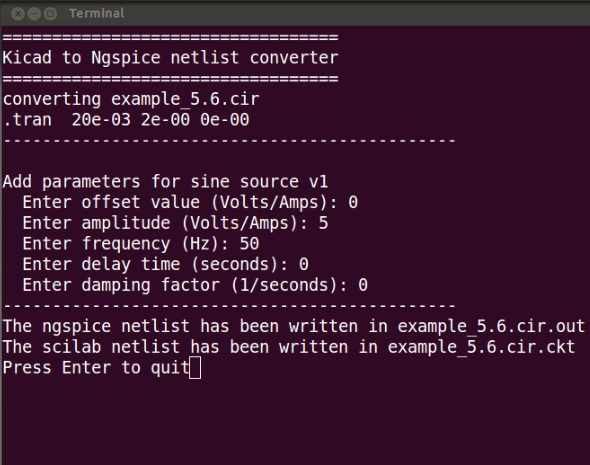
\includegraphics[width=0.7\textwidth]{figures/8}
\caption{Parameters to be added for sinusoidal source}
\label{8}
\end{figure}
- in the terminal the details of sinusoidal source like “offset value”, “amplitude”, “frequency”, delay time”, “damping factor” are asked. This is shown in Figure \ref{8}.
\item When DC source of unknown value is available in schematic
\begin{figure}[t]
\centering
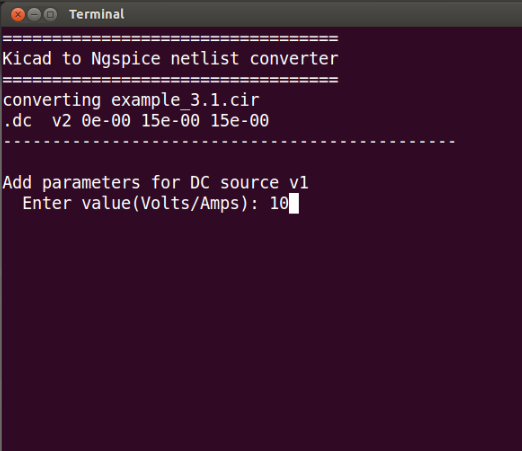
\includegraphics[width=0.7\textwidth]{figures/9}
\caption{Parameters to be added for dc source}
\label{9}
\end{figure}
- It will ask for the value of DC source. In the example shown in Figure \ref{9}, the value of DC source is 10V.
\item When AC source is available in schematic
\begin{figure}[t]
\centering
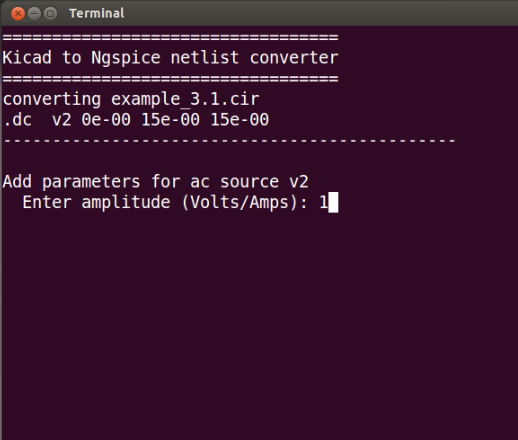
\includegraphics[width=0.7\textwidth]{figures/10}
\caption{Parameters to be added for ac source}
\label{10}
\end{figure}
- It will ask for amplitude of AC source, which in this case is 1V. This is shown in Figure \ref{10}.
\end{enumerate}
\subsection{Convert IC into discrete blocks}
As Eeschema (schematic editor used in Oscad) is intended for PCB Designing, it creates netlist in terms of IC and not components, e.g., if the circuit contains a two-input Nand gate, then in the netlist, IC 7400 appears instead of the Nand gate. Oscad netlist converter converts the IC into discrete blocks by considering proper input and output connections and IC specifications (voltage levels, speed of the operation etc.). 
\subsection{Insert Digital-to-Analog (D-to-A) and Analog-to-Digital (A-to-D) converter at appropriate places}
Oscad provides capability to perform mixed mode simulation. Thus circuits with analog and digital components can be analyzed. In order to simulate such kind of circuits, D-to-A and A-to-D converters are inserted at appropriate places. The netlist generated from Eeschema is assumed to have analog connections and for digital components, A-to-D converter for inputs and D-to-A converter for outputs are added.
\subsection{Insert plotting and printing statements}\index{plotting and printing statements}
There is a library for plotting and printing the voltages and currents in the circuit. The netlist converter adds appropriate printing and plotting commands (current or voltage plot, or single or differential plot) in the netlist depending on the print/plot components. Ngspice can find the current through voltage sources only. Netlist converter inserts a zero volt voltage source in series with the component through which current needs to be computed. Thus current through any component can be obtained.
\subsection{Insert analysis and option}\index{analysis option}
Oscad netlist converter inserts analysis information created in Section \ref{ana} into the netlist.
\subsection{Insert models and subcircuits}\index{models and subcircuits}
Oscad netlist converter inserts models or subcircuits for required components into the netlist. To know more about model building and subcircuit creation, please refer Chapter \ref{chap8}.
\subsection{Simulation} \index{Simulation}
After netlist conversion, a {\tt .cir.out} file will be generated which is compatible with Ngpice simulation software. Let us see how to simulate this file and obtain the results.
\subsubsection{Ngspice simulation in Oscad} \index{Ngspice simulation}
Click on Ngspice from the Oscad toolbar.  The Ngspice terminal and waveform windows will appear. An example is shown in Figure \ref{11}.
\begin{figure}[t]
\centering
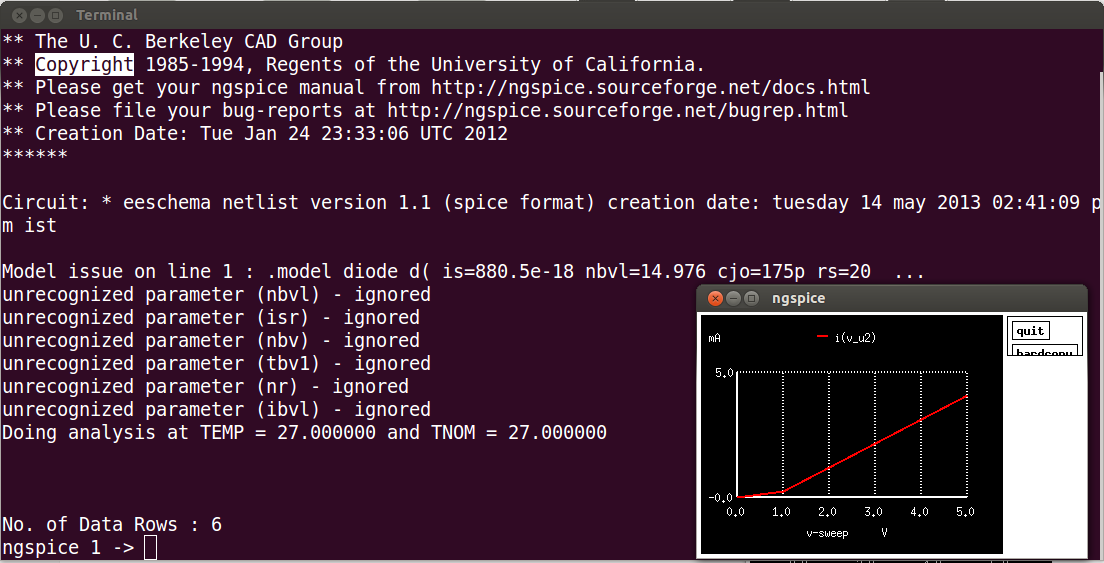
\includegraphics[width=\textwidth]{figures/11}
\caption{Ngspice simulation of {\tt .cir.out} file}
\label{11}
\end{figure}
\section{Examples}
Let us see a few simulation examples \index{simulation examples} which describes the use of Analysis inserter, Netlist converter and Ngspice.
\subsection{DC Analysis} \index{DC Analysis}
\label{dc}
Consider the {\tt nodalExample} (nodal analysis) given in the {\tt Examples} folder available in the Oscad webpage   {\tt www.oscad.net}. Open Schematic editor and generate spice netlist as shown in Chapter \ref{chap5}. Click on ``analysis inserter". Here we decide which type of analysis we want to do. Let us do {\tt DC Analysis}.

  Click on DC  and Enter the following details:

 {\tt source name} = i1, {\tt start} = 0A, {\tt Increment} = 1A, {\tt stop} = 10A and then click on Add Simulation data. You get the window as shown in Figure \ref{12}. Save and close the analysis.
\begin{figure}[t]
\centering
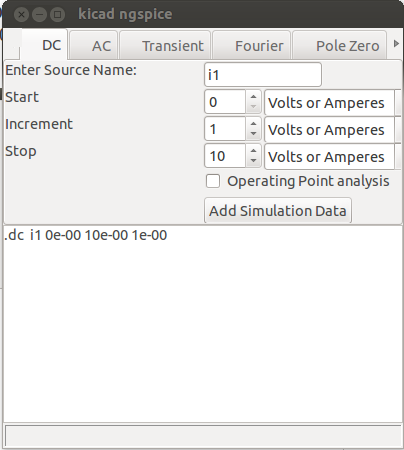
\includegraphics[width=0.5\textwidth]{figures/12}
\caption{DC analysis -- adding simulation data}
\label{12}
\end{figure}
Now click on Netlist Converter which shows the  terminal given in Figure \ref{13}. Press `enter' key.
\begin{figure}[t]
\centering
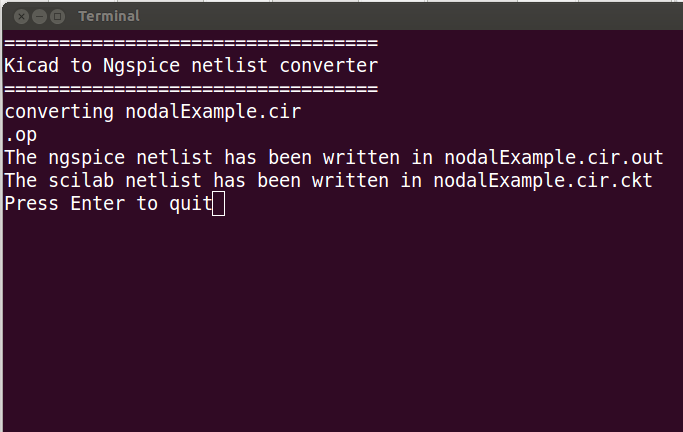
\includegraphics[width=0.7\textwidth]{figures/13}
\caption{Terminal - KiCad to Ngspice netlist converter}
\label{13}
\end{figure}
After this click on Ngspice tool which will show Ngspice terminal with waveform window as shown in the Figure \ref{14}.
\begin{figure}[t]
\centering
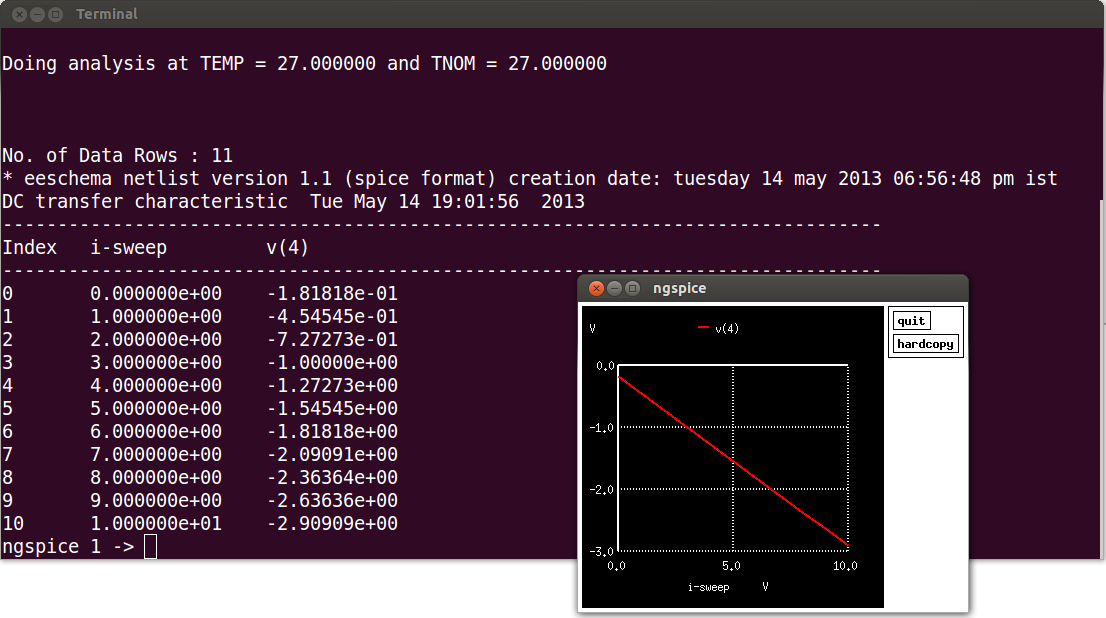
\includegraphics[width=\textwidth]{figures/14}
\caption{Ngspice simulation result}
\label{14}
\end{figure}
\subsection{AC Small-signal Analysis}\index{AC Small-signal Analysis}
Consider the {\tt RC\_ac} example from the {\tt Example} folder available in Oscad website. Open Schematic editor and generate spice netlist as given in Chapter \ref{chap5}. Click on ``analysis inserter". Let us do {\tt AC Analysis}.

Click on {\tt AC} and add the following details: ``scale" = lin, ``start frequency" = 1 Hz, ``stop frequency" = 10 Meg, ``number of points" = 10 and then click on Add simulation data. This is shown in Figure \ref{15}.
\begin{figure}[t]
\centering
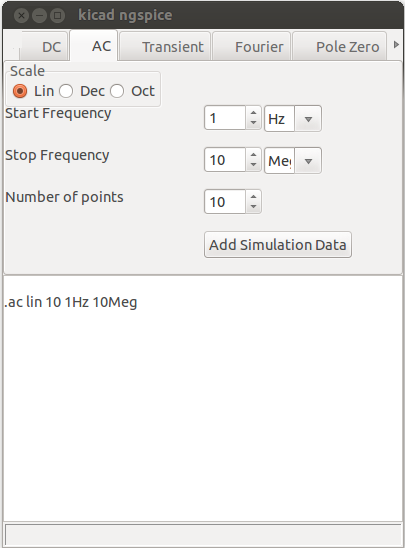
\includegraphics[width=0.5\textwidth]{figures/5}
\caption{AC analysis inserter}
\label{15}
\end{figure}
Now click on Netlist converter which opens up a terminal. It asks for the amplitude of AC. Type {\tt 1} and press 'enter' key. A {\tt .cir.out} netlist file is generated.   This is shown in Figure \ref{16}.
\begin{figure}[t]
\centering
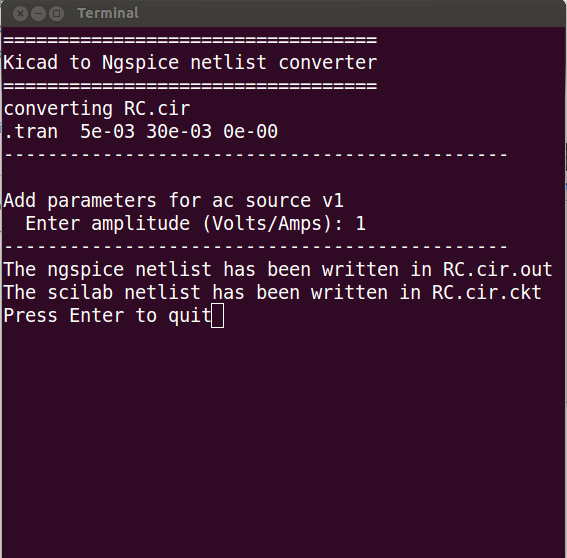
\includegraphics[width=0.5\textwidth]{figures/16}
\caption{AC analysis - Netlist converter}
\label{16}
\end{figure}
After this click on Ngspice tool which will show Ngspice terminal with waveform window as shown in following figure \ref{17}.
\begin{figure}[t]
\centering
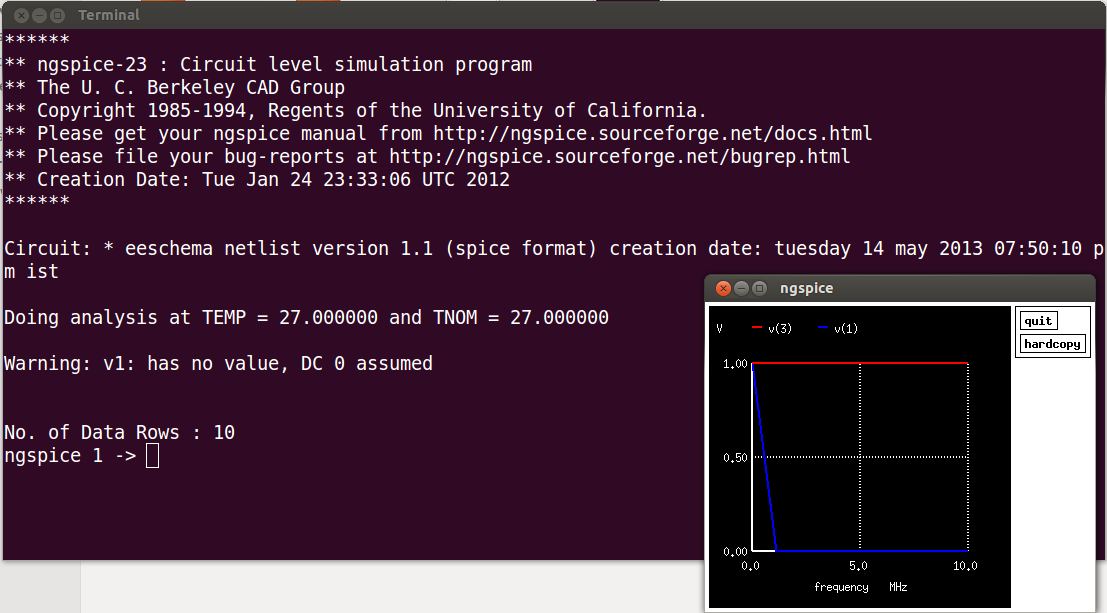
\includegraphics[width=\textwidth]{figures/17}
\caption{AC analysis example - simulation results}
\label{17}
\end{figure}
\subsection{Transient Analysis}\index{Transient Analysis}
Let us use the RC circuit project created in Chapter \ref{chap5} to do transient simulation. Open the {\tt Anlaysis inserter} tool.
Click on transient and then add the following details:

``start time" = 0 sec, ``step time" = 1 ms,``stop time" = 20 ms and then click on Add simulation data. This is shown in Figure \ref{18}.
\begin{figure}[t]
\centering
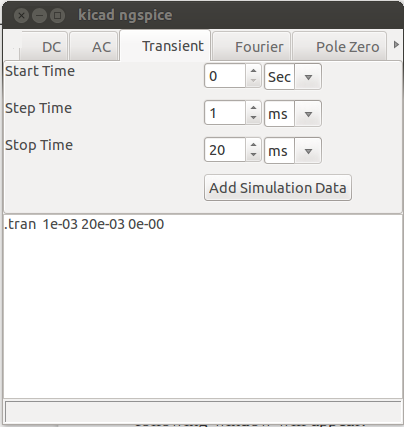
\includegraphics[width=0.5\textwidth]{figures/18}
\caption{Transient analysis inserter}
\label{18}
\end{figure}
Now click on Netlist converter which opens up a terminal. It asks for various parameters for the sine source. Enter the details as given below:

{\tt Offset value} = 0, {\tt Amplitude} = 1, {\tt frequency} = 50, {\tt delay time} = 0, {\tt damping factor} = 0 and press `Enter' key.  This is shown in Figure \ref{19}.
\begin{figure}[t]
\centering
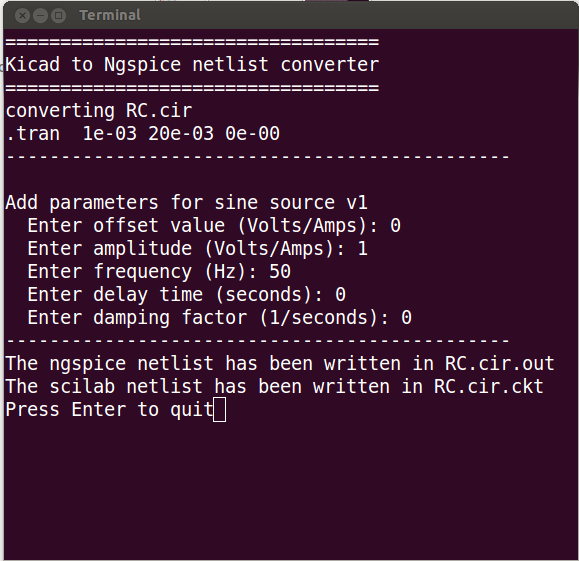
\includegraphics[width=0.7\textwidth]{figures/19}
\caption{Transient analysis -Netlist converter}
\label{19}
\end{figure}
Now click on Ngspice tool which will shows Ngspice terminal with waveform window as shown in following figure \ref{20}.
\begin{figure}[t]
\centering
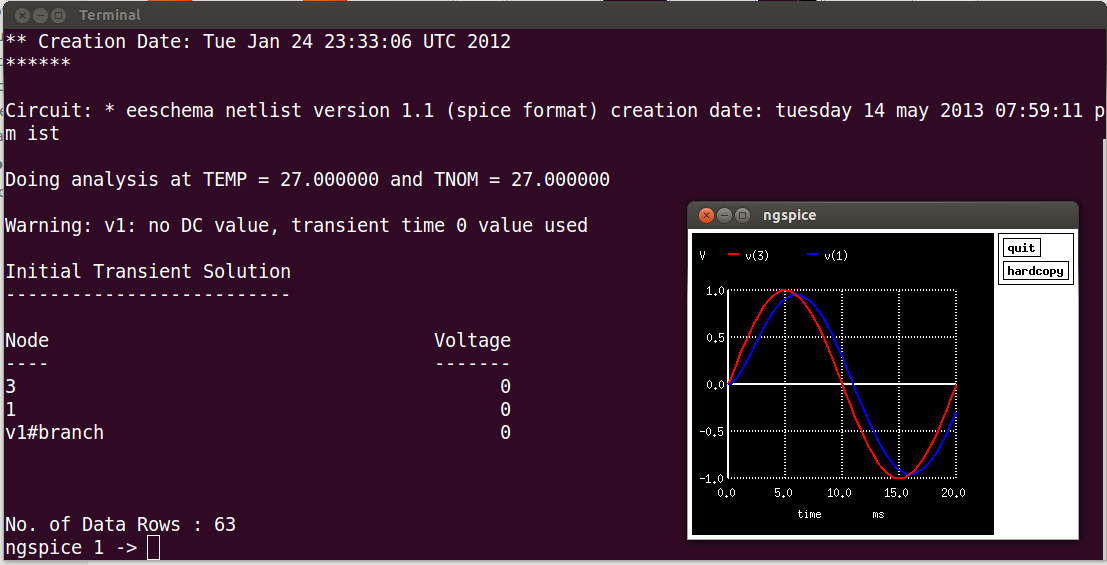
\includegraphics[width=\textwidth]{figures/20}
\caption{Transient analysis example - simulation results}
\label{20}
\end{figure}
